\section{Introduction}
In the paper \cite{huberman_evolutionary_1993} the authors showed that the results of simulating the classic prisoners-dilemma game on a 2D-grid as reported in \cite{nowak_evolutionary_1992} depends on a a very specific strategy of iterating this simulation and show that the beautiful patterns seen in figure \ref{fig:sync_patterns} will not form when selecting a different iteration-strategy.

\begin{figure}[H]
	\centering
  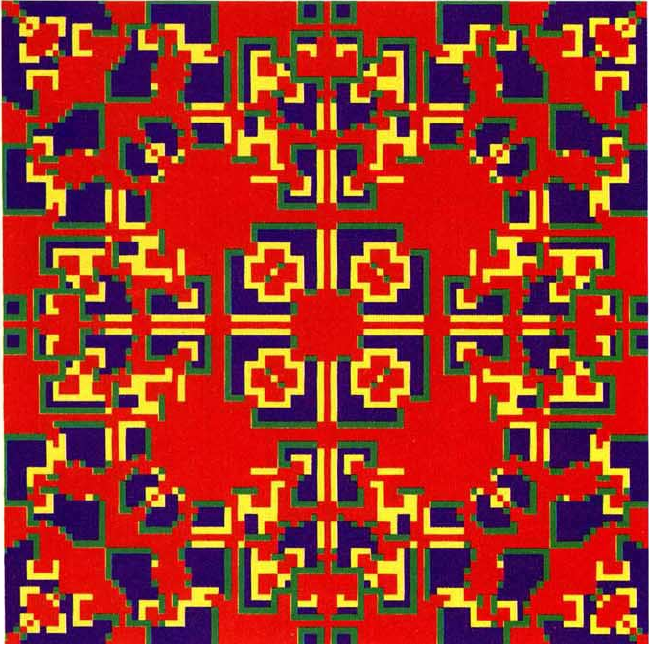
\includegraphics[width=.4\textwidth, angle=0]{./fig/sync_patterns.png}
	\caption{Patterns formed by playing the prisoners-dilemma game on a 2D-grid using a \textit{synchronous} update-strategy. Picture taken from \cite{huberman_evolutionary_1993}.}
	\label{fig:sync_patterns}
\end{figure}

Although the authors differentiated between two strategies, their description still lacks precision which we will try to give in this paper. Although they too discussed philosophical aspects of choosing one strategy over the other, they lacked to generalize their observation. We will do so in the central message of our paper by stressing that when doing ABS \textit{it is of most importance to select the right iteration-strategy which reflects and supports the corresponding semantics of the model}. We find that this awareness is yet still under-represented in the literature of ABS and lacking a systematic treatment. Thus our contribution in this paper is to provide a such by
\begin{itemize}
	\item Presenting general properties of ABS and deriving update-strategies.
	\item Developing a new, general terminology of talking about the update-strategies.
	\item Giving the semantic interpretation and meaning of each of them.
	\item Comparing the three programming languages Java, Haskell and Scala with Actors in regard of their suitability to implement each of these strategies.
\end{itemize}

It is important to note that the amount of research of using Haskell in the field of ABS has so far been moderate. Though there exist a few papers which look into Haskell and ABS \cite{de_jong_suitability_2014}, \cite{sulzmann_specifying_2007}, \cite{jankovic_functional_2007} all treat Haskell in this context very generally and focus primarily on how to specify Agents. This papers is looking at fundamental technical details of Haskell's suitability in implementing update-strategies in ABS, something not looked at in the ABS community thus presenting an original novelty.

TODO \cite{sorokin_aivika_2015}